\section{Verschiedene Versionen der Anzeige}
\setauthor{Oliver Sugic}
Für die graphische Oberfläche wurden verschiedene Ideen und Konzepte ausprobiert, um die Benutzbarkeit für die Lernenden und Lehrenden zu optimieren.
Im Laufe des Kapitels wird erläutert, welche Versionen der Anzeige es gab und welche Versionen sich als sinnvoll erwiesen haben.

\subsection{Version 1: Visualisierung mit Karten}
\setauthor{Oliver Sugic}
Am Anfang wurden Überlegungen angestellt, wie man die Lernenden als auch die Lehrenden am besten in nicht vertrautes Gebiet führen kann.
Da die meisten Person mit Kartenservices, wie beispielsweise Google Maps oder ähnlichen Dienstleistungen, vertraut sind, wurde eine Karte implementiert.
Es gibt viele verschiedene Anbieter von Kartenservices, die in Betracht gezogen wurde. 
Da Google Maps eines der bekanntesten Anbieter, wurde auf die Google Maps Api gesetzt. 
Doch im Laufe der Recherche ist klar geworden, dass die Google Maps Api nicht die beste Lösung für dieses Projekt ist  aus folgenden Gründen: \cite{Ashraf}
\begin{itemize}
    \item Die Google Maps Api läuft über die Google Cloud und ist daher kostenpflichtig
    \item Google Maps Api ist nicht open-source
    \item Google Maps Api ist nicht einfach zu anzupassen an die Bedürfnisse des Projektes 
\end{itemize}


Auf der Suche nach weiteren Alternativen, verwies mich Herr Pavelescu auf die Open-Source Kartenlösung Leaflet.
Leaflet ist eine JavaScript Libary, die es ermöglicht, Karten in Webanwendungen zu integrieren. \cite{Agafonkin} 


\pagebreak

\begin{lstlisting}[numbers=left,language=HTML,caption={Implementierung einer Karte mit Leaflet},label={lst:leafletmap}]{}
    <style>
    #map { height: 1000px; }
    </style>
    </head>
    <body>
     <link rel="stylesheet" href="https://unpkg.com/leaflet@1.9.3/dist/leaflet.css"
         integrity="sha256-kLaT2GOSpHechhsozzB+flnD+zUyjE2LlfWPgU04xyI="
         crossorigin=""/>
    
     <script src="https://unpkg.com/leaflet@1.9.3/dist/leaflet.js"
         integrity="sha256-WBkoXOwTeyKclOHuWtc+i2uENFpDZ9YPdf5Hf+D7ewM="
         crossorigin=""></script>
    
     <div id="map"></div>
      <script>
    var map = L.map('map').setView([48.2684159, 14.2517532], 20);
    L.tileLayer('https://tile.openstreetmap.org/{z}/{x}/{y}.png', {
        maxZoom: 19,
        attribution: '&copy; <a href="http://www.openstreetmap.org/copyright">OpenStreetMap</a>'
    }).addTo(map);
    </script> 
\end{lstlisting}

\begin{figure}[h]
\centering
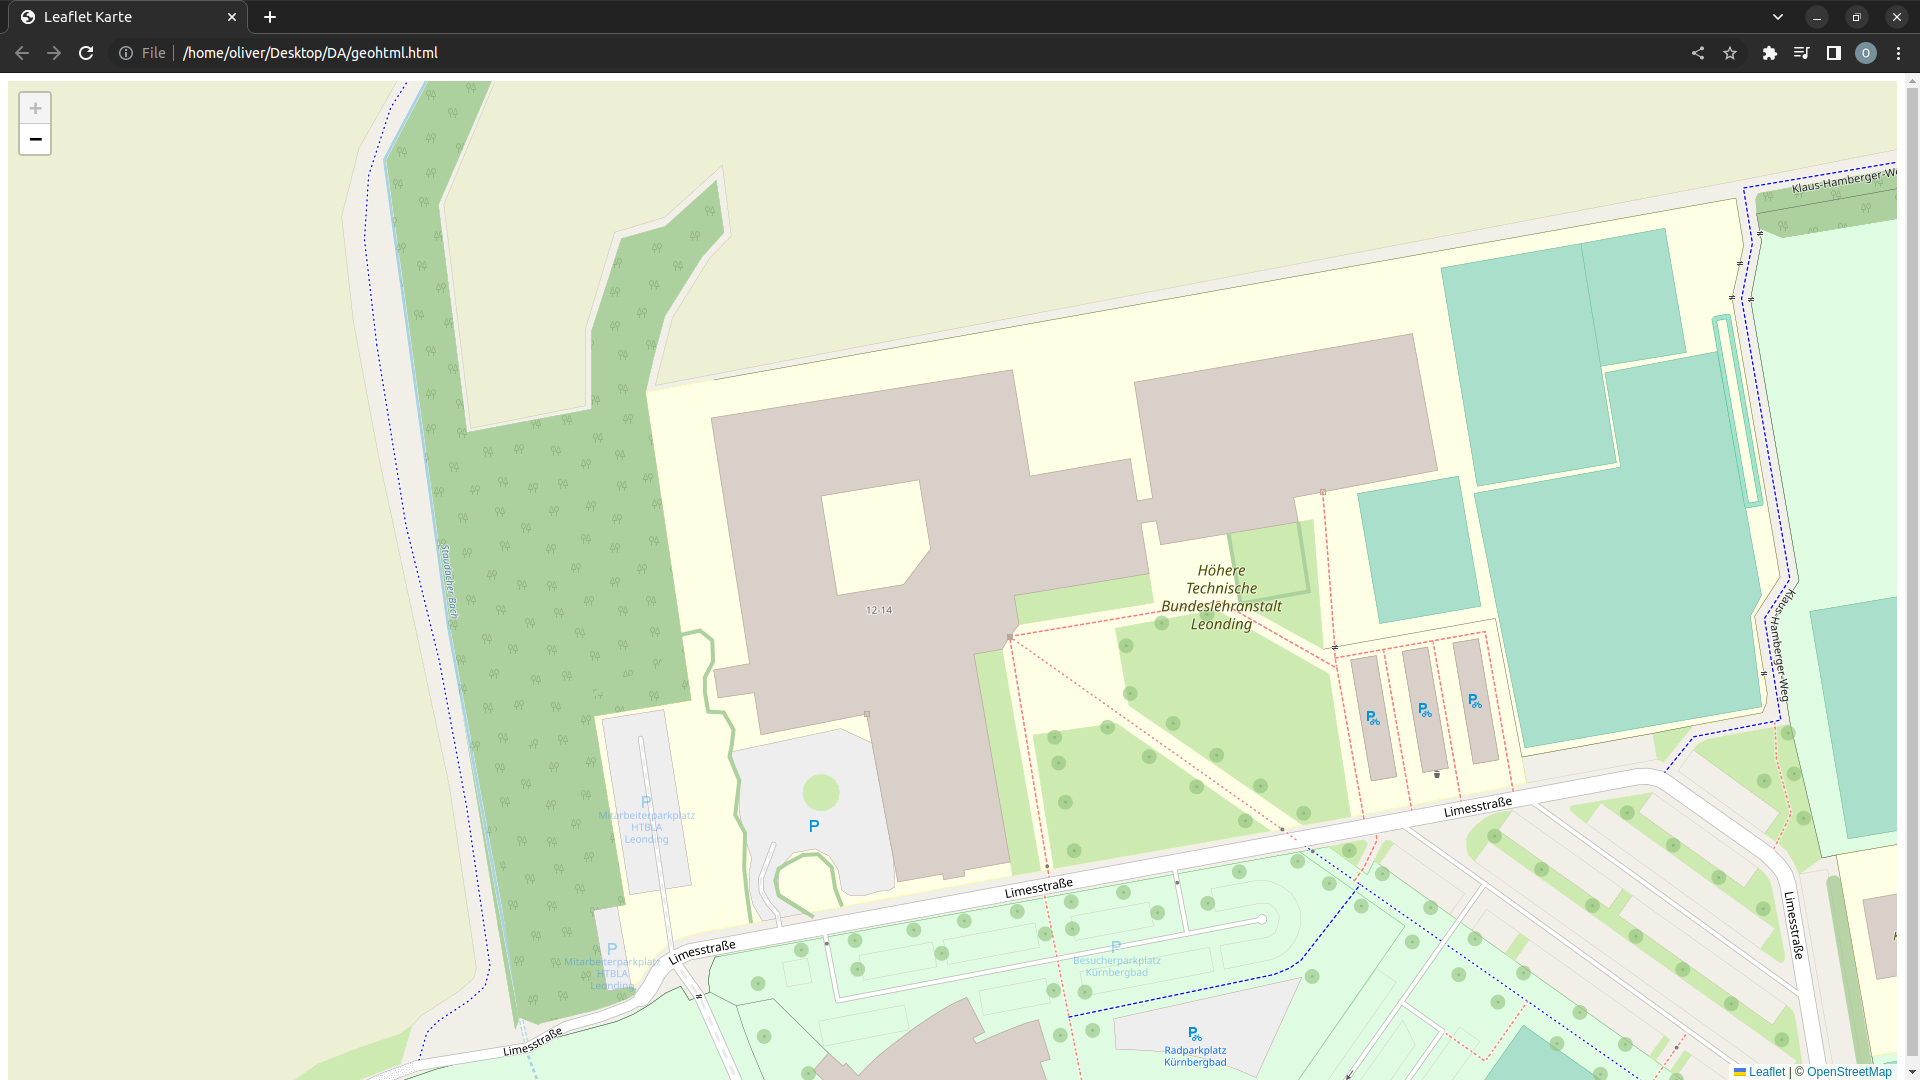
\includegraphics[scale=0.2]{pics/leafletmap.png}
\caption{Ergebnis der Implementierung mit Leaflet}
\end{figure}


\subsection{Version 2: Leaflet Karte mit Routing}
\setauthor{Oliver Sugic}
Nach dem ersten Prototypen mit Leaflet, wurde die Idee weiter verfolgt, um die Benutzerfreundlichkeit für die Teilnehmenden zu verbessern. Eine Route vom eigenen Standort zur nächsten Aktivität wurde implementiert. Um die Routen anzeigen zu können, wurde die Leaflet Routing Machine verwendet. 
Hierfür wird das Plugin Leaflet Routing Machine verwendet, das ebenfalls vom Leaflet zur Verfügung gestellt wird. Mit dieser Erweiterung Können Routen zwischen zwei Punkten auf der Karte berechnet werden und angezeigt werden. Ebenfalls können die Wegpunkte einfach geändert werden.\cite{Liedman2015}  

\begin{lstlisting}[numbers=left,language=HTML,caption={Implementierung einer Karte mit Leaflet Routing Engine},label={lst:leafletmap}]
<head>
    <title>Leaflet Karte</title>
    <style>
        #map {
            height: 1500px;
        }
    </style>
</head>

<body>
    <link rel="stylesheet" href="https://unpkg.com/leaflet@1.9.3/dist/leaflet.css"
        integrity="sha256-kLaT2GOSpHechhsozzB+flnD+zUyjE2LlfWPgU04xyI=" crossorigin="" />

    <script src="https://unpkg.com/leaflet@1.9.3/dist/leaflet.js"
        integrity="sha256-WBkoXOwTeyKclOHuWtc+i2uENFpDZ9YPdf5Hf+D7ewM=" crossorigin="">
        </script>
    <link rel="stylesheet" href="https://unpkg.com/leaflet@1.2.0/dist/leaflet.css" />
    <link rel="stylesheet" 
    href="https://unpkg.com/leaflet-routing-machine@latest/dist/leaflet-routing-machine.css" />
    <script 
    src="https://unpkg.com/leaflet@1.2.0/dist/leaflet.js"></script>
    <script src="https://unpkg.com/leaflet-routing-machine@latest/dist/leaflet-routing-machine.js"></script>

    <div id="map"></div>
    <script>
        var map = L.map('map').setView([48.2684159, 14.2517532], 15);
        L.tileLayer('https://tile.openstreetmap.org/{z}/{x}/{y}.png', {
            maxZoom: 19,
            attribution: '&copy; <a href="http://www.openstreetmap.org/copyright">OpenStreetMap</a>'
        }).addTo(map);
        L.Routing.control({
            waypoints: [
                L.latLng(48.2684159, 14.2517532),
                L.latLng(48.2627373, 14.2589871)
            ]
        }).addTo(map);
    </script>
</body>
\end{lstlisting}

\begin{figure}[h]
    \centering
    \includegraphics[scale=0.15]{pics/Leaflet_Routing.png}
    \caption{Ergebnis der Implementierung mit Leaflet Routing Machine}
\end{figure}

Allerding traten bei der Implementierung Probleme auf. Das Plugin konnte nicht die Route darstellen, was auf einen Fehler in der Implementierung zurückzuführen war.

\subsection{Version 3: Angular Geoloaction API}
\setauthor{Oliver Sugic}
Da die Implementierung mit der Leaflet Routing Machine nicht funktioniert hat, wurde versucht, mittels des Standorts des Nutzenden zur nächsten Aktivität zu navigieren. 

\section{Aktuelle Komponenten}
\setauthor{Oliver Sugic}
Derzeit besteht die Anwendung aus drei Komponenten. In diesem Kapitel werden der Aufbau und und Zusammenhänge der einzelnen Komponenten erläutert.  

\subsection{Angular Frontend}
\setauthor{Oliver Sugic}
Der schwierigste Teil der Arbeit liegt darin, eine Benutzeroberfläche zu erstellen, die einfach zu bedienen aber auch ansprechend für den Benutzer ist.
Es wurde daher auf das Angular Framework genommen, da es sehr 

\subsubsection{Schüler Sicht}

Nach dem Scheitern der Implementierung mit der Leaflet Routing Machine, wurde eine neues Design entworfen, um die Benutzerfreundlichkeit zu verbessern.
Nach vielen Überlegung wurde ein Wireframe entworfen \ref{lst:Wireframe}, welches sowohl für mobile Endgeräte geeignet ist, aber auch überschaubar für die nutzenden Personen ist.

\begin{figure}[h]
    \centering
    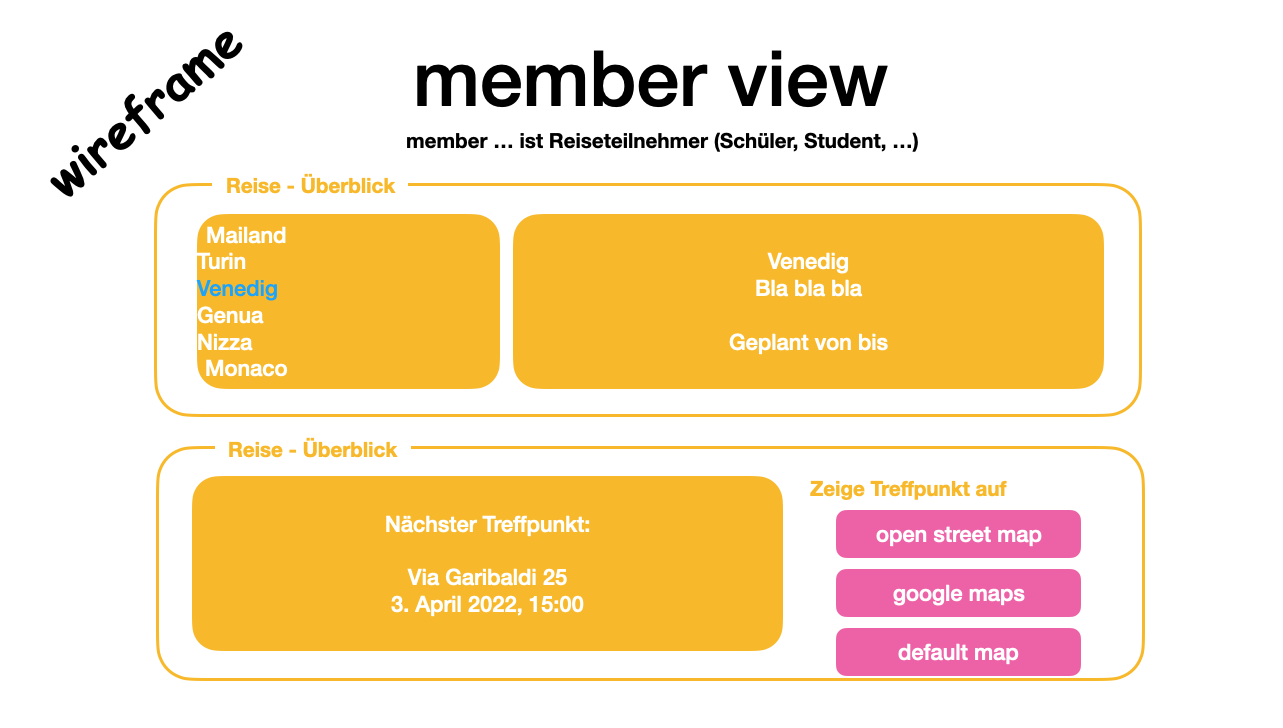
\includegraphics[scale=0.3]{pics/Wireframe.png}
    \caption{Endgültige Version }
    \label{lst:Wireframe}
\end{figure}


Der Nutzer soll in einen groben Überblick haben, welche Städte er besuchen wird. Durch eine kurze Beschreibung der Aktivität solle der Reisende einen kurzen Einblick haben, was Ihn erwarten wird. In der unteren Hälfte des Bildschirm erhält man genauere Informationen über den Treffpunkt, außerdem ist es möglich sich auf der Karte die Route anzeigen zu lassen. Es ist möglich, sich auf der standartmäßigen Karte des Endgeräts, über Google Maps oder über die OpenStreetMap zu navigieren. Der Nutzende kann für sich entscheiden, welche Karte Ihm am besten gefällt oder welche Karte Ihm am meisten vertraut ist wie in Abbildung \ref{lst:Overview} zu sehen ist.

\begin{figure}[h]
    \centering
    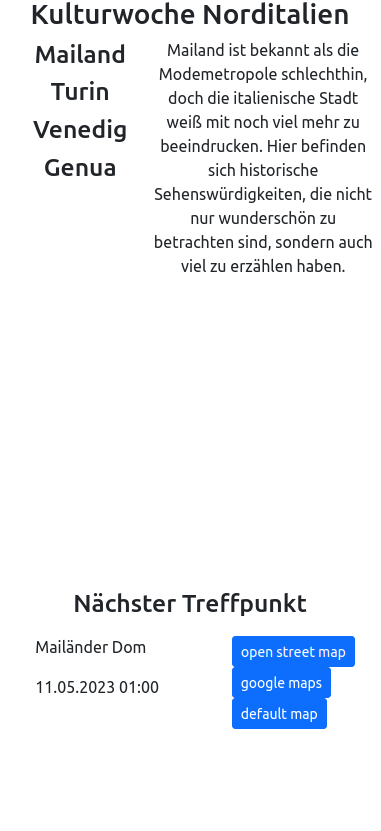
\includegraphics[scale=0.8]{pics/overview.png}
    \caption{Schüler Ansicht}
    \label{lst:Overview}
\end{figure}

\newpage

Da den Schüler und Schülerinnen die Mitführung von elektronischen Geräten, müssen die Schüler und Schülerinnen Ihre Handys benutzen, da die Mitführung eines Handys nicht verboten ist. Somit musste die Ansichten für mobil Geräte angepasst werden. 

\subsubsection{Aktivitäten freischalten}
Um die Aktivitäten freizuschalten, kann der Lehrer über die Unlock-Activity Komponente die Aktivitäten freischalten. Es werden alle Aktivitäten angezeigt und kann durch bedienen des Buttons freigeschaltet werden oder auch wieder gesperrt werden.

\begin{figure}[h]
    \centering
    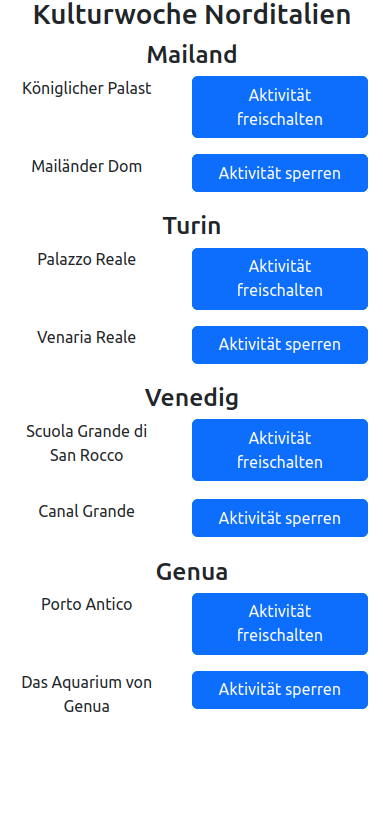
\includegraphics[scale=0.8]{pics/unlock-activity.png}
    \caption{Aktivitäten freischalten und sperren}
    \label{lst:UnlockActivity}
\end{figure}

Wieder musste auf die mobile Ansicht geachtet werden. Die Lehrer oder die Lehrerinnen haben zwar einen Laptop mit, aber da es sehr unpraktisch ist mit einem Laptop durch unbekanntes Gebiet herumzureisen, wurde die Ansicht für mobile Geräte angepasst. 

\subsubsection{Event erstellen}
Für das erstellen eines Events wurde eine eigene Komponente entworfen und entwickelt. Da eine Lehrkraft in die Reise im voraus planen muss, ist sie für den Gebrauch von Laptops angepasst worden.

Die Komponente wurde in vier Abschnitte geteilt:

\begin{itemize}
    \item Daten des Events
    \item Daten der Teilnehmer 
    \item Daten des Themas
    \item Daten der Aktivitäten
\end{itemize}

\begin{figure}[h]
    \centering
    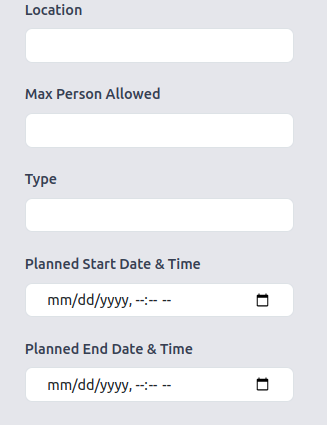
\includegraphics[scale=0.35]{pics/create-event.png}
    \caption{Abschnitt für die Daten des Events}
    \label{lst:event}
\end{figure}

\begin{figure}[h]
    \centering
    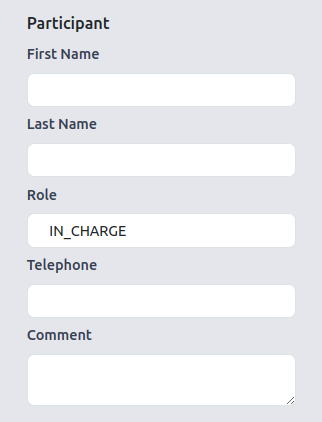
\includegraphics[scale=0.35]{pics/add-participant.png}
    \caption{Abschnitt für die Daten der Teilnehmer}    
    \label{lst:participant}
\end{figure}

\begin{figure}[h]
    \centering
    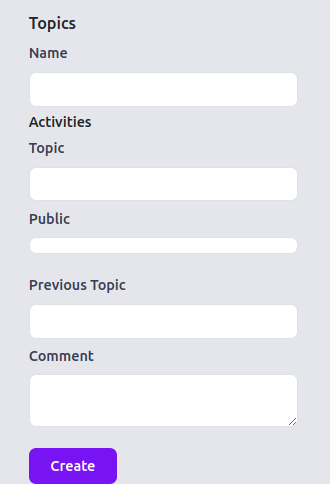
\includegraphics[scale=0.35]{pics/add-topic.png}
    \caption{Abschnitt für die Daten des Themas}
    \label{lst:topic}
\end{figure}

\begin{figure}[h]
    \centering
    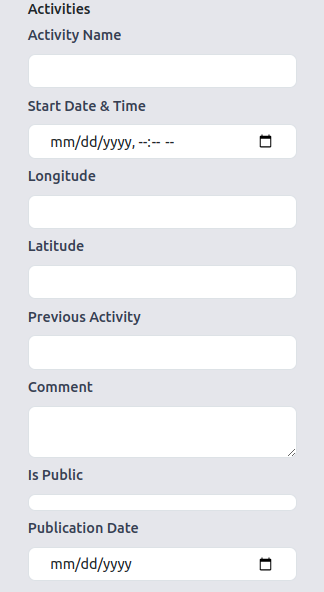
\includegraphics[scale=0.35]{pics/add-activites.png}
    \caption{Abschnitt für die Daten der Aktivitäten}
    \label{lst:activity}
\end{figure}

\newpage

\subsection{Quarkus Backend}
\setauthor{Oliver Sugic}

Für die Verwaltung der Daten wurde ein Backend entwickelt.


\subsection{Keycloak}
\setauthor{Oliver Sugic}

\subsection{Deployment}
\setauthor{Oliver Sugic}

\subsection{Mögliche zukünftige Erweiterungen}
\setauthor{Oliver Sugic}


